%%
\begin{frame}
    \frametitle{Elementi interventi editoriali}
    \addtocounter{nframe}{1}
    
    %\begin{center}
    %    
\includegraphics[width=.2\textwidth]{../imgs/tei-r.pdf}
    %\end{center}

    \begin{block}{Testo aggiunto, cancellato, lacunoso}
        \begin{itemize}
            \item \texttt{<add>} \textbf{una o più parole aggiunte nel testo}
            \item[] \texttt{questa parola è <add place="supralinear" >stata</add> aggiunta in un secondo momento}
        \end{itemize}
        
    \end{block}
    
\end{frame}

\begin{frame}
    \frametitle{Elementi interventi editoriali}
    \addtocounter{nframe}{1}
    
    %\begin{center}
    %    
\includegraphics[width=.2\textwidth]{../imgs/tei-r.pdf}
    %\end{center}

    \begin{block}{Testo aggiunto, cancellato, lacunoso}
        \begin{itemize}
            \item \texttt{<del>} \textbf{una o più parole cancellate nel testo}
            \item[] \texttt{questa invece era <del rend="overstrike" >era</del> di troppo e l’ho cancellata}
        \end{itemize}
        
    \end{block}
    
\end{frame}


\begin{frame}
    \frametitle{Elementi interventi editoriali}
    \addtocounter{nframe}{1}
    
    %\begin{center}
    %    
\includegraphics[width=.2\textwidth]{../imgs/tei-r.pdf}
    %\end{center}

    \begin{block}{Testo aggiunto, cancellato, lacunoso}
        \begin{itemize}
            \item \texttt{<gap />} \textbf{parte di testo omessa, mancante o illeggibile}
            \item[] \texttt{questa <gap reason="illegible" extent="6" unit="chars"/> è illeggibile (forse "parola"?)}
        \end{itemize}
        
    \end{block}
    
\end{frame}



%%
\begin{frame}
    \frametitle{Elementi interventi editoriali}
    \addtocounter{nframe}{1}
    
    %\begin{center}
    %    
\includegraphics[width=.2\textwidth]{../imgs/tei-r.pdf}
    %\end{center}

    \begin{block}{Testo danneggiato, poco chiaro, inserito dal curatore}
        \begin{itemize}
            \item \texttt{<damage>} \textbf{testo danneggiato nel documento originale}
            \item[] \texttt{per qualche goccia d’acqua questa parola si è <damage agent="water" >scolorita</damage> molto}
        \end{itemize}
        
    \end{block}
    
\end{frame}

\begin{frame}
    \frametitle{Elementi interventi editoriali}
    \addtocounter{nframe}{1}
    
    %\begin{center}
    %    
\includegraphics[width=.2\textwidth]{../imgs/tei-r.pdf}
    %\end{center}

    \begin{block}{Testo danneggiato, poco chiaro, inserito dal curatore}
        \begin{itemize}
            \item \texttt{<unclear>} \textbf{parte di testo interpretabile con difficoltà}
            \item[] \texttt{<unclear reason="faded" >questa</unclear> si legge
            ancora ma con difficoltà}
        \end{itemize}
        
    \end{block}
    
\end{frame}

\begin{frame}
    \frametitle{Elementi interventi editoriali}
    \addtocounter{nframe}{1}
    
    %\begin{center}
    %    
\includegraphics[width=.2\textwidth]{../imgs/tei-r.pdf}
    %\end{center}

    \begin{block}{Testo danneggiato, poco chiaro, inserito dal curatore}
        \begin{itemize}
            \item \texttt{<supplied>} \textbf{testo inserito dal curatore perché illeggibile nell’originale o assente}
            \item[] \texttt{qui <supplied>mancava qualcosa</supplied> nel testo}
        \end{itemize}
        
    \end{block}

    \textit{\texttt{<supplied>}  (fa parte del modulo transcr)}

\end{frame}

%è possibile combinare questi elementi (compreso <gap/>)

%%
\begin{frame}
    \frametitle{Elementi interventi editoriali}
    \addtocounter{nframe}{1}
    
    %\begin{center}
    %    
\includegraphics[width=.2\textwidth]{../imgs/tei-r.pdf}
    %\end{center}

    \begin{block}{Dal Vercelli Book}
         \begin{center}
            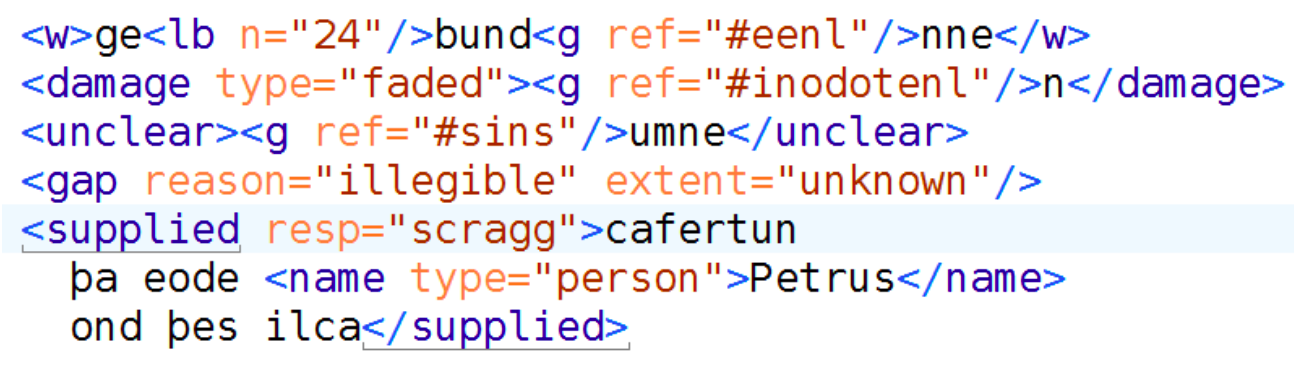
\includegraphics[width=.9\textwidth]{imgs/vercelli.png}
        \end{center}
    \end{block}
    \textit{Manoscritto in inglese antico, dialetto tardo sassone occidentale, X secolo ca.}

\end{frame}
  

%%
\begin{frame}
    \frametitle{Elementi interventi editoriali}
    \addtocounter{nframe}{1}
    
    %\begin{center}
    %    
\includegraphics[width=.2\textwidth]{../imgs/tei-r.pdf}
    %\end{center}

    \begin{block}{Elemento sostituzione}
        Può succedere che una parola non sia semplicemente cancellata, ma che sia anche sostituita da un altro termine
    \end{block}
    \begin{block}{Elemento sostituzione}
        In questo caso è possibile usare l’elemento \texttt{<subst>} per collegare la sequenza cancellazione - nuovo testo
    \end{block}
    \texttt{<subst>} fa parte del modulo transcr, per ulteriori informazioni \texttt{(@seq)} v. \url{http://www.tei-c.org/release/doc/tei-p5-doc/en/html/PH.html\#PHSU}
\end{frame}


%%
\begin{frame}
    \frametitle{Elementi interventi editoriali}
    \addtocounter{nframe}{1}
    
    %\begin{center}
    %    
\includegraphics[width=.2\textwidth]{../imgs/tei-r.pdf}
    %\end{center}

    \begin{block}{Elemento sostituzione: parola}
        \texttt{questa parola è stata <subst> <del rend="overstrike" >scritta</del> <add place="supralinear" >aggiunta</add> </subst> in un secondo momento}
    \end{block}

    \begin{block}{Elemento sostituzione: carattere}
        \texttt{<subst><del rend="overtype" >t<del><add>T</add></subst>i scrivo una     mail domani mattina}
    \end{block}
   
\end{frame}




%%
\begin{frame}
    \frametitle{Elementi interventi editoriali}
    \addtocounter{nframe}{1}
    
    %\begin{center}
    %    
\includegraphics[width=.2\textwidth]{../imgs/tei-r.pdf}
    %\end{center}

    \begin{block}{Attributi e valori consigliati}
        \begin{itemize}
            \item \texttt{<add>} \textbf{place} \textit{inline, supralinear, margin} \textbf{hand} \textit{author, scribe1, scribe2}
            \item \texttt{<del>} \textbf{rend} \textit{overstrike, subpunct, overtype, dotted} \textbf{hand} \textit{author, scribe1, scribe2}
            \item \texttt{<gap>} \textbf{reason} \textit{illegible, cancelled, irrelevant, missing, omissis, censored} \textbf{hand} \textit{editor} \textbf{agent} \textit{water, smoke, hole, missing page} \textbf{extent} \textit{chars, words, cm}
            \item \texttt{<unclear>} \textbf{reason} \textit{parterased, ink blot} \textbf{hand} \textit{author, scribe1, scribe2} \textbf{agent} \textit{water, smoke, ink}
        \end{itemize}
    \end{block}
    
\end{frame}

%%
\begin{frame}
    \frametitle{Elementi interventi editoriali}
    \addtocounter{nframe}{1}
    
    %\begin{center}
    %    
\includegraphics[width=.2\textwidth]{../imgs/tei-r.pdf}
    %\end{center}

    \begin{block}{Correzioni e normalizzazioni}
        \begin{itemize}
            \item \texttt{<sic>} \textbf{parola o frase ritenuta errata, ma riportata così come appare scritta}
            \item[] \texttt{questa parola è <sic>statta</sic> sbagliata}
        \end{itemize}
        
    \end{block}
    
\end{frame}

\begin{frame}
    \frametitle{Elementi interventi editoriali}
    \addtocounter{nframe}{1}
    
    %\begin{center}
    %    
\includegraphics[width=.2\textwidth]{../imgs/tei-r.pdf}
    %\end{center}

    \begin{block}{Correzioni e normalizzazioni}
        \begin{itemize}
            \item \texttt{<corr>} \textbf{correzione di una parola o frase errata}
            \item[] \texttt{questa parola è <corr>stata</corr> corretta in un secondo momento}
        \end{itemize}
        
    \end{block}
    
\end{frame}

\begin{frame}
    \frametitle{Elementi interventi editoriali}
    \addtocounter{nframe}{1}
    
    %\begin{center}
    %    
\includegraphics[width=.2\textwidth]{../imgs/tei-r.pdf}
    %\end{center}

    \begin{block}{Correzioni e normalizzazioni}
        \begin{itemize}
            \item \texttt{<orig>} \textbf{parola o frase ritenuta non standard}
            \item[] \texttt{Allora, mi dici <orig>'ndo</orig> vai?}
        \end{itemize}
        
    \end{block}
    
\end{frame}

\begin{frame}
    \frametitle{Elementi interventi editoriali}
    \addtocounter{nframe}{1}
    
    %\begin{center}
    %    
\includegraphics[width=.2\textwidth]{../imgs/tei-r.pdf}
    %\end{center}

    \begin{block}{Correzioni e normalizzazioni}
        \begin{itemize}
            \item \texttt{<reg>} \textbf{parola o frase normalizzata (regularised)}
            \item[] \texttt{Allora, mi dici <reg>dove</reg> vai?}
        \end{itemize}
        
    \end{block}
    
\end{frame}

%%
\begin{frame}
    \frametitle{Elementi interventi editoriali}
    \addtocounter{nframe}{1}
    
    %\begin{center}
    %    
\includegraphics[width=.2\textwidth]{../imgs/tei-r.pdf}
    %\end{center}

    \begin{block}{Abbreviazioni ed espansioni}
        \begin{itemize}
            \item \texttt{<abbr>} \textbf{parola abbreviata, brevigrafo}
            \item[] \texttt{chiedi al <abbr>dott.</abbr> Rossi}
            \item[] \texttt{in nomine Patris <abbr>7</abbr> Filii
            <abbr>7</abbr> Spiritus Sancti}
        \end{itemize}
        
    \end{block}
    
\end{frame}

\begin{frame}
    \frametitle{Elementi interventi editoriali}
    \addtocounter{nframe}{1}
    
    %\begin{center}
    %    
\includegraphics[width=.2\textwidth]{../imgs/tei-r.pdf}
    %\end{center}

    \begin{block}{Abbreviazioni ed espansioni}
        \begin{itemize}
            \item \texttt{<expan>} \textbf{espansione di un’abbreviazione}
            \item[] \texttt{chiedi al <expan>dottor</expan> Rossi}
            \item[] \texttt{in nomine Patris <expan>et</expan> Filii <expan>et</expan> Spiritus Sancti}
        \end{itemize}
        
    \end{block}
    
\end{frame}

 %%

 \begin{frame}
    \frametitle{Elementi interventi editoriali}
    \addtocounter{nframe}{1}
    
    %\begin{center}
    %    
\includegraphics[width=.2\textwidth]{../imgs/tei-r.pdf}
    %\end{center}

    \begin{block}{Abbreviazioni ed espansioni}
        \begin{itemize}
            \item \texttt{<abbr>} \textbf{usare l’attributo type per specificare il tipo}
            \item[] \texttt{chiedi al <abbr type="titolo" >dott.</abbr> Rossi}
            \item[] \texttt{in nomine Patris <abbr type="brevigrafo" >7</abbr> Filii <abbr type="brevigrafo" >7</abbr> Spiritus}
        \end{itemize}
        
    \end{block}
    
\end{frame}

\begin{frame}
    \frametitle{Elementi interventi editoriali}
    \addtocounter{nframe}{1}
    
    %\begin{center}
    %    
\includegraphics[width=.2\textwidth]{../imgs/tei-r.pdf}
    %\end{center}
    \textit{Disponibili ulteriori elementi aggiungendo il modulo transcr:}
    \begin{block}{Abbreviazioni ed espansioni}
        \begin{itemize}
            \item \texttt{<am>} \textbf{lettere o segni di abbreviazione}
            \item \texttt{<ex>} \textbf{lettere aggiunte espandendo un’abbreviazione}
            \item[] \texttt{<abbr>sanct<am>\texttt{u\~{}}</am></abbr>}
            \item[] \texttt{ <expan>sanctu<ex>m</ex></expan>}
        \end{itemize}
        
    \end{block}
    
\end{frame}
 

 %%
 \begin{frame}
    \frametitle{Elementi interventi editoriali}
    \addtocounter{nframe}{1}
    
    %\begin{center}
    %    
\includegraphics[width=.2\textwidth]{../imgs/tei-r.pdf}
    %\end{center}

    \textit{Alcuni elementi di intervento editoriale sono perfettamente speculari}
    \begin{block}{Elementi speculari}
        \begin{itemize}
            \item \texttt{<sic> - <corr>} 
            \item \texttt{<orig> - <reg>}
            \item \texttt{<abbr> - <expan>}
        \end{itemize}
        
    \end{block}
    
\end{frame}

%%
\begin{frame}
    \frametitle{Elementi interventi editoriali}
    \addtocounter{nframe}{1}
    
    %\begin{center}
    %    
\includegraphics[width=.2\textwidth]{../imgs/tei-r.pdf}
    %\end{center}

    \begin{block}{Elemento choice}
        Nella \textit{TEI P5} è stato introdotto un nuovo elemento \texttt{<choice>} che comprende ogni coppia
    \end{block}
    \begin{block}{Elemento choice}
        La relazione fra le coppie è importante per essere sicuri che ciascun elemento sia collegato all’altro
    \end{block}
\end{frame}

%%
\begin{frame}
    \frametitle{Elementi interventi editoriali}
    \addtocounter{nframe}{1}
    
    %\begin{center}
    %    
\includegraphics[width=.2\textwidth]{../imgs/tei-r.pdf}
    %\end{center}
    \textit{Disponibili ulteriori elementi aggiungendo il modulo transcr:}
    \begin{block}{Coppie in choice}
        \begin{itemize}
            \item \texttt{<sic> - <corr>} 
            \item[] \texttt{questa parola è <choice> <sic>statta</sic> <corr>stata</corr> </choice> scritta sbagliata}
        \end{itemize}
        
    \end{block}
    
\end{frame}

\begin{frame}
    \frametitle{Elementi interventi editoriali}
    \addtocounter{nframe}{1}
    
    %\begin{center}
    %    
\includegraphics[width=.2\textwidth]{../imgs/tei-r.pdf}
    %\end{center}
    \textit{Disponibili ulteriori elementi aggiungendo il modulo transcr:}
    \begin{block}{Coppie in choice}
        \begin{itemize}
            \item \texttt{<orig> - <reg>} 
            \item[] \texttt{Allora, mi dici <choice><orig>’ndo</orig> <reg>dove</reg></choice> vai?}
        \end{itemize}
        
    \end{block}
    
\end{frame}

\begin{frame}
    \frametitle{Elementi interventi editoriali}
    \addtocounter{nframe}{1}
    
    %\begin{center}
    %    
\includegraphics[width=.2\textwidth]{../imgs/tei-r.pdf}
    %\end{center}
    \textit{Disponibili ulteriori elementi aggiungendo il modulo transcr:}
    \begin{block}{Coppie in choice}
        \begin{itemize}
            \item \texttt{<abbr> - <expan>} 
            \item[] \texttt{chiedi al <choice><abbr>dott.</abbr> <expan>dott<ex>or</ex></expan></choice> Rossi}
        \end{itemize}
        
    \end{block}
    
\end{frame}

%%
\begin{frame}
    \frametitle{Elementi interventi editoriali}
    \addtocounter{nframe}{1}
    
    %\begin{center}
    %    
\includegraphics[width=.2\textwidth]{../imgs/tei-r.pdf}
    %\end{center}

    \begin{block}{Attributi responsabilità}
        Per \texttt{<add> e <del>} abbiamo l’attributo \texttt{@hand} per specificare, se necessario, \textbf{l’autore} della \textbf{modifica} all’originale
    \end{block}
    \begin{block}{Attributi responsabilità}
        Per qualche intervento editoriale, invece, potrebbe essere importante specificare il \textbf{responsabile} (in particolare per l’elemento \texttt{<supplied>}!) e il grado di \textbf{certezza}
    \end{block}
    \textbf{Per fare questo si usano gli attributi @resp e @cert}
\end{frame}


%%

\begin{frame}
    \frametitle{Elementi interventi editoriali}
    \addtocounter{nframe}{1}
    
    %\begin{center}
    %    
\includegraphics[width=.2\textwidth]{../imgs/tei-r.pdf}
    %\end{center}

    \begin{block}{Attributi responsabilità}
        \texttt{questa parola è <choice> <sic>statta</sic> <corr resp="amdg" >stata</corr> </choice> scritta per errore}
    \end{block}
    \textit{Il valore di \texttt{@resp} può rimandare a un \texttt{<respStmt>}}
    \texttt{<corr resp="\#amdg" >stata</corr>}
\end{frame}


%%

\begin{frame}
    \frametitle{Elementi interventi editoriali}
    \addtocounter{nframe}{1}
    
    %\begin{center}
    %    
\includegraphics[width=.2\textwidth]{../imgs/tei-r.pdf}
    %\end{center}
    \begin{block}{Altri elementi utili}
        \begin{itemize}
            \item \texttt{<gb/>} \textbf{gathering begins}
            \item[] \textit{indica l’inizio di un nuovo fascicolo nella trascrizione di un manoscritto}
        \end{itemize}
        
    \end{block}
    
\end{frame}

\begin{frame}
    \frametitle{Elementi interventi editoriali}
    \addtocounter{nframe}{1}
    
    %\begin{center}
    %    
\includegraphics[width=.2\textwidth]{../imgs/tei-r.pdf}
    %\end{center}
    \begin{block}{Altri elementi utili}
        \begin{itemize}
            \item \texttt{<space>} \textbf{modulo linking}
            \item[] \textit{usato per marcare la presenza di spazio significativo (ad esempio spazio lasciato dallo scriba per inserire una iniziale miniata)}
            \item[] normalmente usato come elemento vuoto
        \end{itemize}
        
    \end{block}
    
\end{frame}

\begin{frame}
    \frametitle{Elementi interventi editoriali}
    \addtocounter{nframe}{1}
    
    %\begin{center}
    %    
\includegraphics[width=.2\textwidth]{../imgs/tei-r.pdf}
    %\end{center}
    \begin{block}{Altri elementi utili}
        \begin{itemize}
            \item \texttt{<pc>} \textbf{modulo analysis}
            \item[] \textit{contiene uno o più caratteri che costituiscono una forma di punteggiatura nel testo}
            \item[] punctuation character(s)
        \end{itemize}
        
    \end{block}
    
\end{frame}


%%
\begin{frame}
    \frametitle{Elementi interventi editoriali}
    \addtocounter{nframe}{1}
    
    %\begin{center}
    %    
\includegraphics[width=.2\textwidth]{../imgs/tei-r.pdf}
    %\end{center}
    \begin{block}{Altri elementi utili}
        \begin{itemize}
            \item \texttt{<ab>} \textbf{anonymous block}
            \item[] \textit{contenitore di testo simile a un paragrafo ma senza il valore semantico di quest’ultimo}
            \item[] modulo linking
        \end{itemize}
        
    \end{block}
    
\end{frame} 

\begin{frame}
    \frametitle{Elementi interventi editoriali}
    \addtocounter{nframe}{1}
    
    %\begin{center}
    %    
\includegraphics[width=.2\textwidth]{../imgs/tei-r.pdf}
    %\end{center}
    \begin{block}{Altri elementi utili}
        \begin{itemize}
            \item \texttt{<seg>} \textbf{arbitrary segment}
            \item[] \textit{usato per marcare qualunque porzione di testo, usare @type per specificare il contenuto semantico}
            \item[] modulo linking
        \end{itemize}
        
    \end{block}
    
\end{frame} 

\begin{frame}
    \frametitle{Elementi interventi editoriali}
    \addtocounter{nframe}{1}
    
    %\begin{center}
    %    
\includegraphics[width=.2\textwidth]{../imgs/tei-r.pdf}
    %\end{center}
    \begin{block}{Altri elementi utili}
        \begin{itemize}
            \item \texttt{<w>} \textbf{word}
            \item[] \textit{marca una parola a livello grammaticale, @lemma per indicare il lemma e @lemmaref per stabilire un link con un dizionario online}
            \item[] modulo analysis
        \end{itemize}
        
    \end{block}
    
\end{frame}

\begin{frame}
    \frametitle{Elementi interventi editoriali}
    \addtocounter{nframe}{1}
    
    %\begin{center}
    %    
\includegraphics[width=.2\textwidth]{../imgs/tei-r.pdf}
    %\end{center}
    \begin{block}{Altri elementi utili}
        \begin{itemize}
            \item \texttt{<c>} \textbf{character}
            \item[] \textit{marca un singolo carattere nel testo}
            \item[] modulo analysis
        \end{itemize}
        
    \end{block}
    
\end{frame} 


%% 
\begin{frame}
    \frametitle{Elementi interventi editoriali}
    \addtocounter{nframe}{1}
    
   
    \begin{block}{Aggiunte scribali}
        \begin{center}
            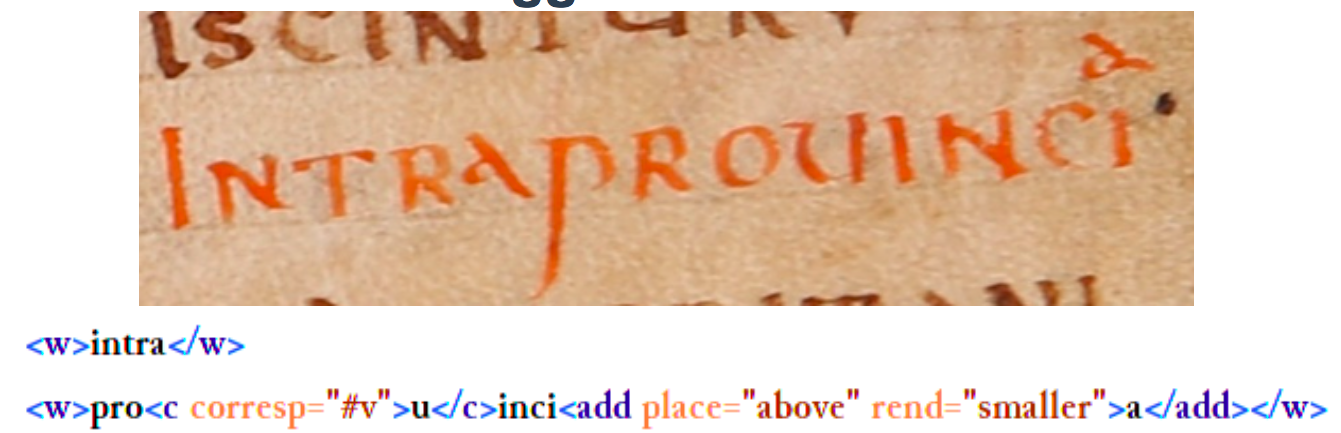
\includegraphics[width=.95\textwidth]{imgs/Aggiunte-1.png}
        \end{center}

    \end{block}
    
\end{frame} 

\begin{frame}
    \frametitle{Elementi interventi editoriali}
    \addtocounter{nframe}{1}
    
   
    \begin{block}{Aggiunte scribali}
        \begin{center}
            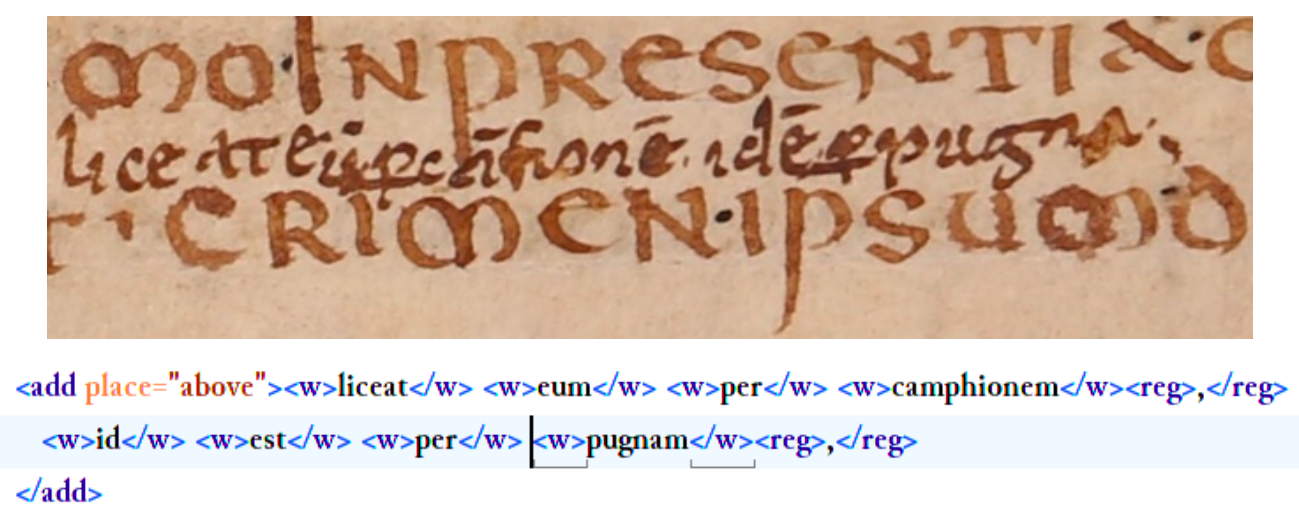
\includegraphics[width=.95\textwidth]{imgs/Aggiunte-2.png}
        \end{center}

    \end{block}
    
\end{frame} 

%%
\begin{frame}
    \frametitle{Elementi interventi editoriali}
    \addtocounter{nframe}{1}
    
    \begin{block}{Cancellature}
        \begin{center}
            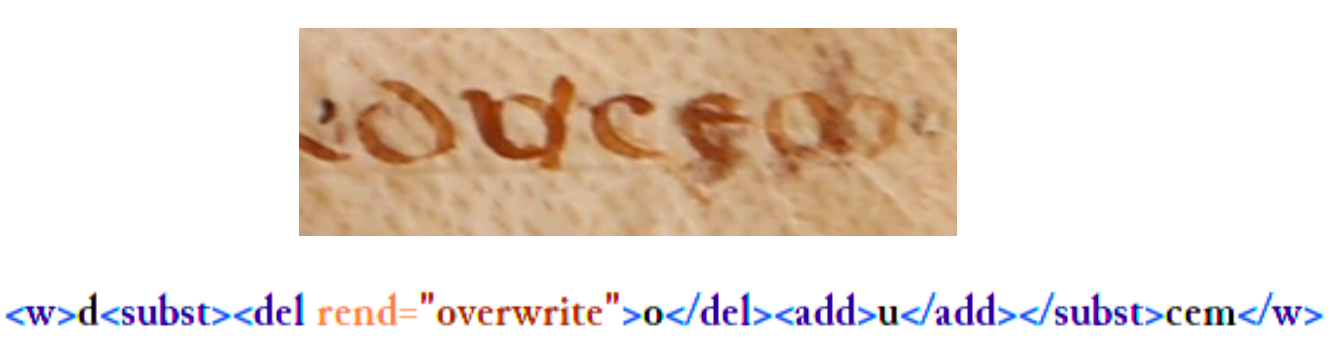
\includegraphics[width=.9\textwidth]{imgs/Cancellature.png}
        \end{center}
    \end{block}
   
    \begin{block}{Cancellature scribali: Dal Vercelli Book}
        \texttt{<del rend="erasure" >ff</del>fore wæron
        <del rend="dot" ><g ref="\#aeligddot"/></del>}
    \end{block}
    
\end{frame} 


\begin{frame}
    \frametitle{Elementi interventi editoriali}
    \addtocounter{nframe}{1}
    
   
    \textit{Abbreviazioni e Espansioni}
        \begin{center}
            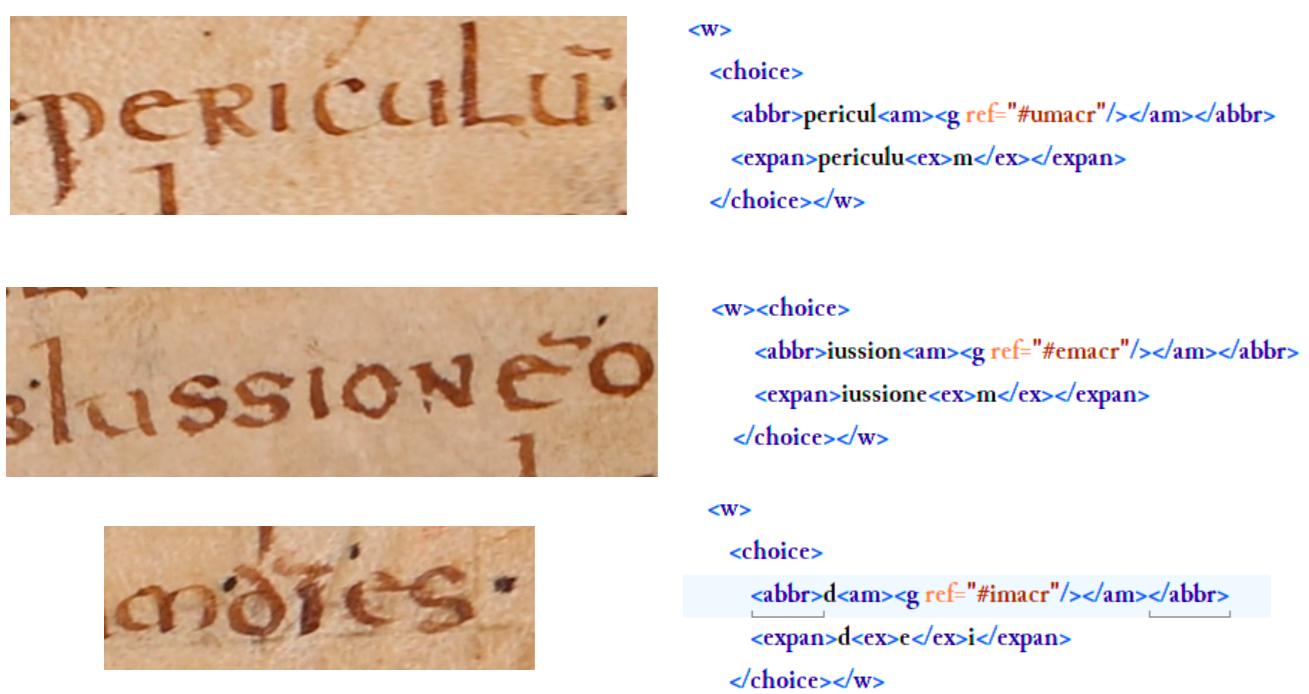
\includegraphics[width=.95\textwidth]{imgs/Abbreviazioni-1.png}
        \end{center}

    
\end{frame}

\begin{frame}
    \frametitle{Elementi interventi editoriali}
    \addtocounter{nframe}{1}
    
   
    \begin{block}{Codifica fenomeni annidati}
        \begin{center}
            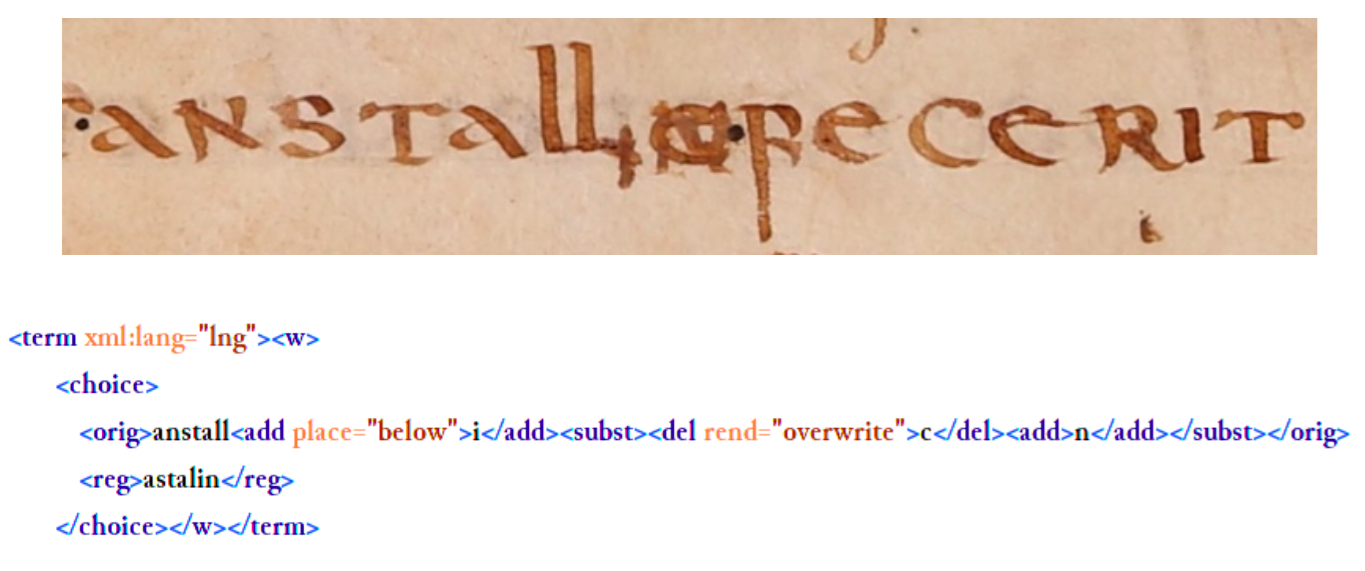
\includegraphics[width=.95\textwidth]{imgs/Aggiunta-cancellatura-regolarizzazione.png}
        \end{center}

    \end{block}
    
\end{frame}

\begin{frame}
    \frametitle{Elementi interventi editoriali}
    \addtocounter{nframe}{1}
    
   
    \begin{block}{Errori Scribali}
        \begin{center}
            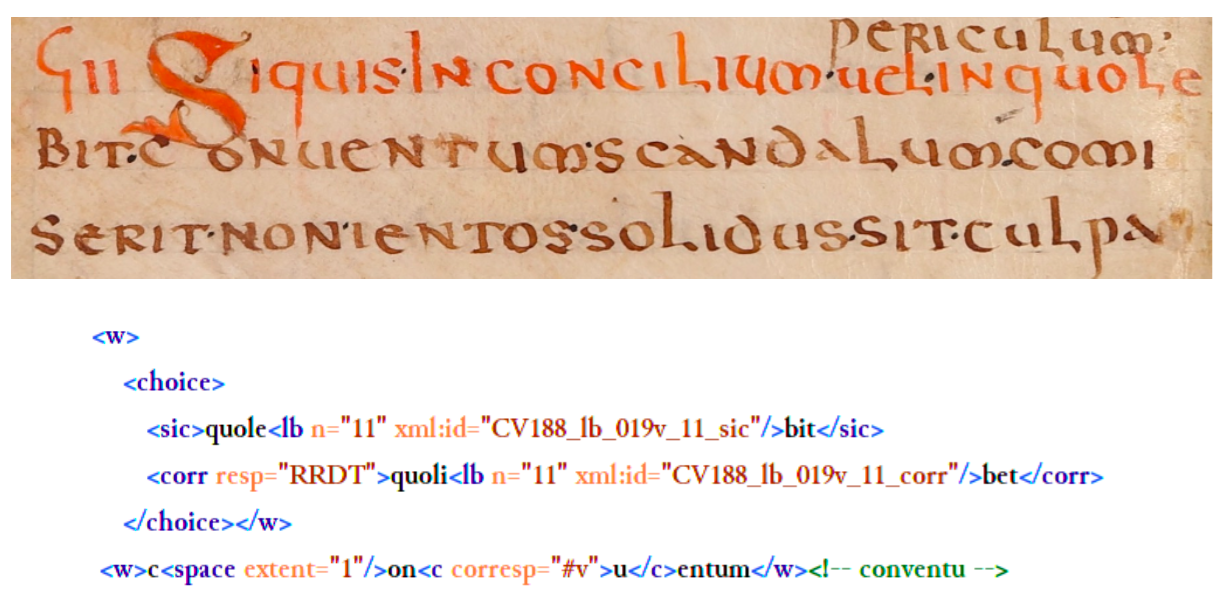
\includegraphics[width=.95\textwidth]{imgs/Correzioni.png}
        \end{center}

    \end{block}
    
\end{frame}

\begin{frame}
    \frametitle{Elementi interventi editoriali}
    \addtocounter{nframe}{1}
        \begin{center}
            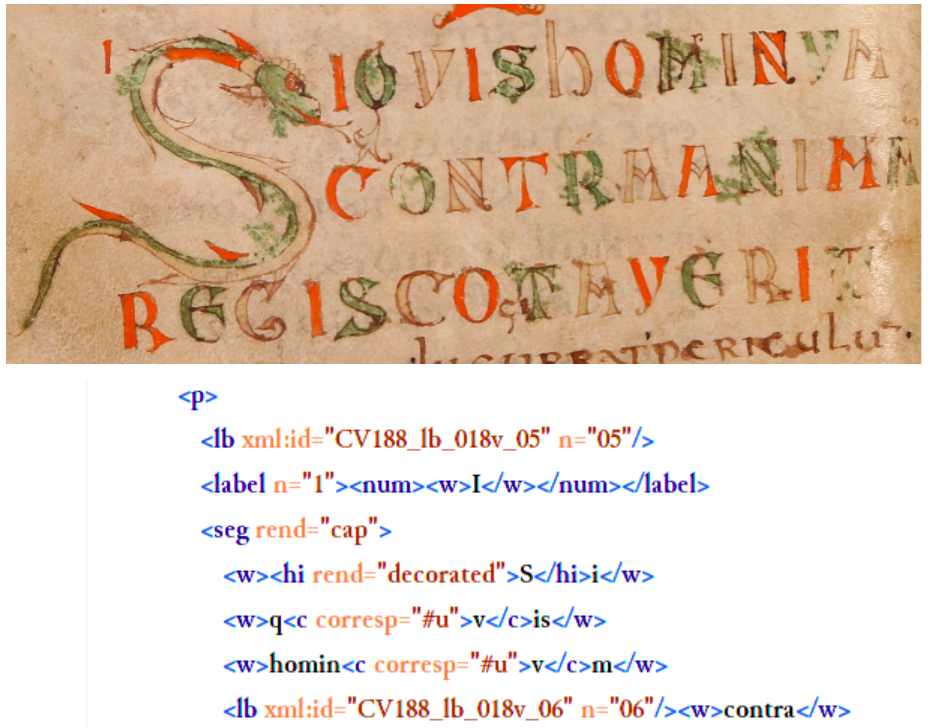
\includegraphics[width=.9\textwidth]{imgs/Decorazioni.png}
        \end{center}
\end{frame}

\begin{frame}
    \frametitle{Elementi interventi editoriali}
    \addtocounter{nframe}{1}
    
    \textit{Marcatura singole parole}
        \begin{center}
            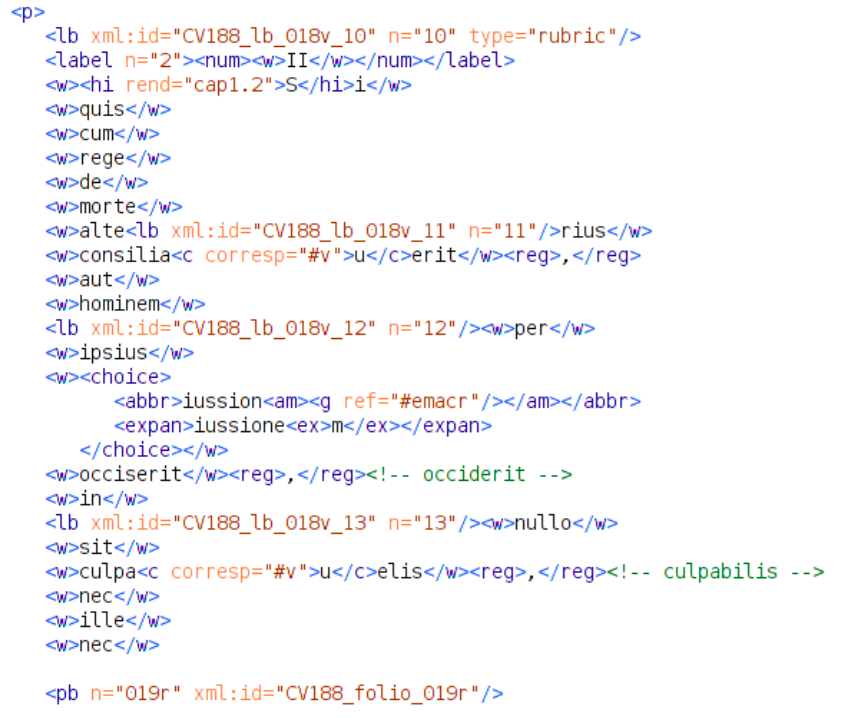
\includegraphics[width=.9\textwidth]{imgs/MarcaturaParole.png}
        \end{center}
    
    
\end{frame}

%% 
\begin{frame}
    \frametitle{Elementi interventi editoriali}
    \addtocounter{nframe}{1}
    
   
    \begin{block}{Esercizio}
        \begin{center}
            Trascrivere e codificare un frammento di lettera di Bellini
            \\(Vincenzo Bellini a Carlo Pepoli, in Puteaux, 26 giugno 1834)
        \end{center}
    \end{block}
    \begin{center}
        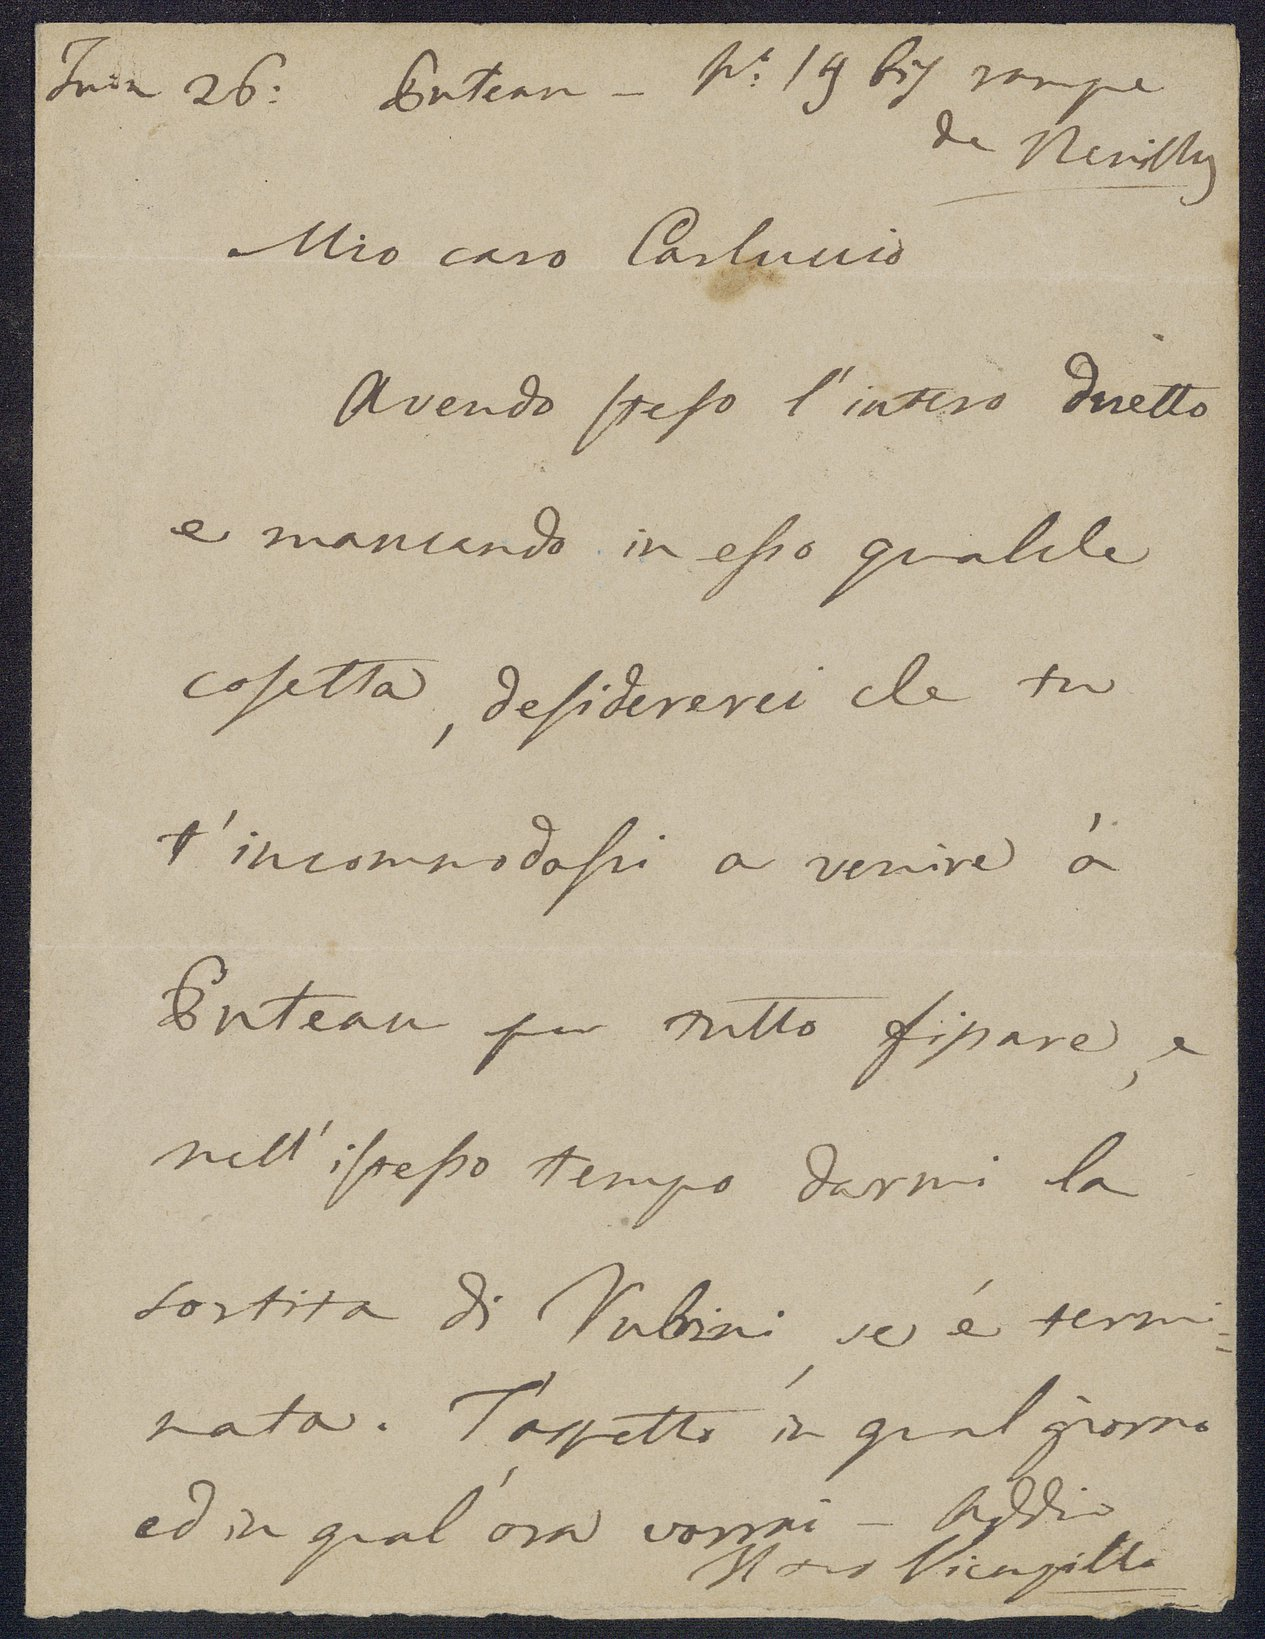
\includegraphics[width=.35\textwidth]{imgs/letteraBellini-1a-LL_1_16.jpg}
    \end{center}
\end{frame}
